\section{Introduction}

\section{Data Set}

\section{Results: Distributed Estimation with Heaviside Basis}

\begin{figure}[h]
\centering
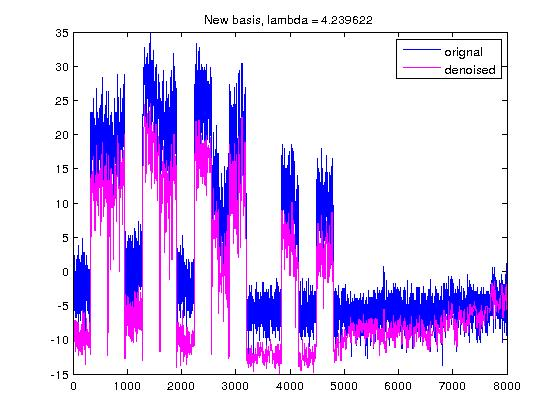
\includegraphics[height = 7.3 cm]{new_basis_ofcom_1.jpg}
\caption{Example of classification with OFCOM data, 35 changepoints}
\label{fig:hvb}
\end{figure}

\begin{figure}[h]
\centering
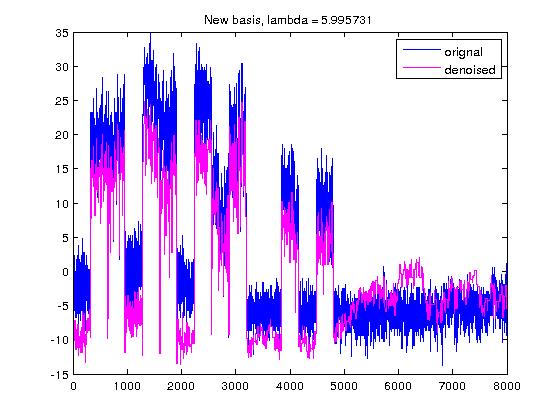
\includegraphics[height = 7.3 cm]{new_basis_ofcom_2.jpg}
\caption{Example of classification with OFCOM data, 55 changepoints}
\label{fig:hvb}
\end{figure}

\begin{figure}[h]
\centering
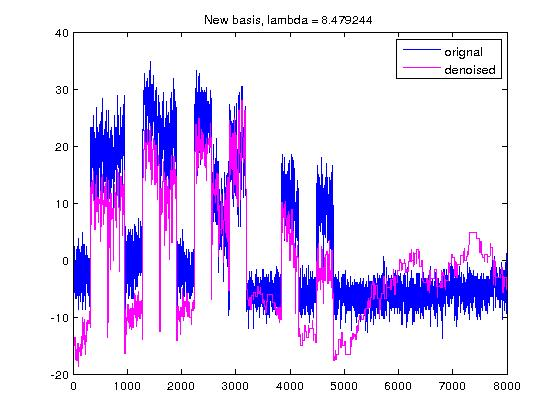
\includegraphics[height = 7.3 cm]{new_basis_ofcom_3.jpg}
\caption{Example of classification with OFCOM data, 35 changepoints}
\label{fig:hvb}
\end{figure}

\begin{figure}[h]
\centering
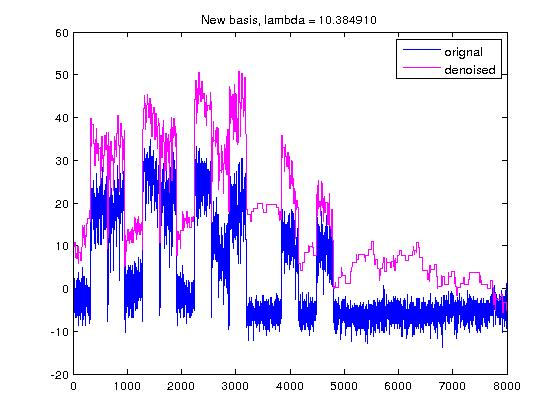
\includegraphics[height = 7.3 cm]{new_basis_ofcom_4.jpg}
\caption{Example of classification with OFCOM data, 55 changepoints}
\label{fig:hvb}
\end{figure}


\section{Compressive Estimation}

Some examples of the output of this procedure are shown below, for synthetic and real (Ofcom) data.

\begin{figure}[h]
\centering
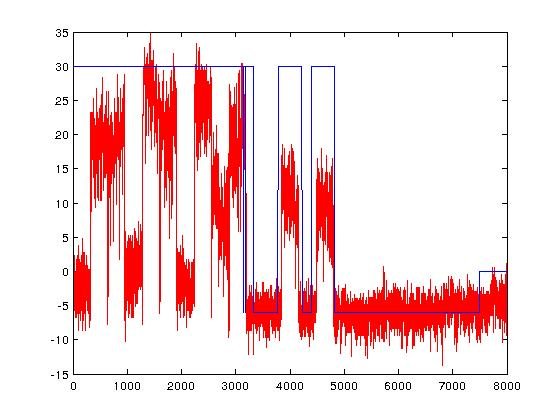
\includegraphics[height = 7.3 cm]{ofcom_classification1.jpg}
\caption{Example of classification with OFCOM data, 35 changepoints}
\label{fig:hvb}
\end{figure}

\begin{figure}[h]
\centering
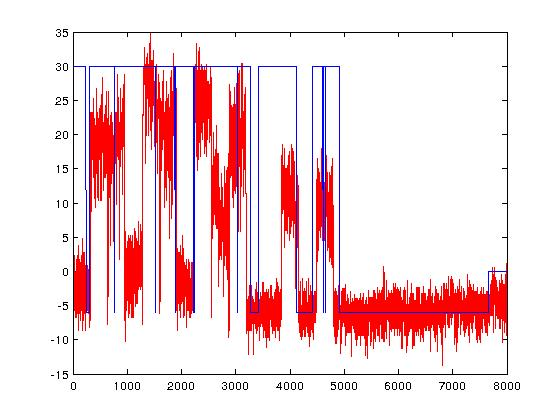
\includegraphics[height = 7.3 cm]{ofcom_classification.jpg}
\caption{Example of classification with OFCOM data, 55 changepoints}
\label{fig:hvb}
\end{figure}

\begin{figure}[h]
\centering
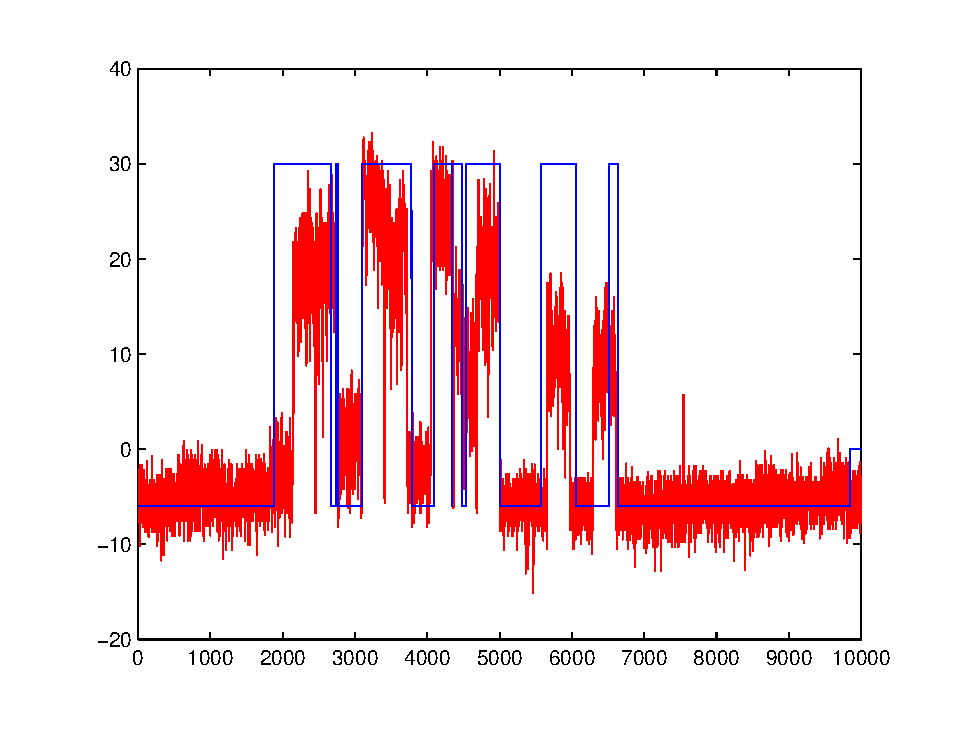
\includegraphics[height = 7.3 cm]{OFCOM5.eps}
\caption{Example of classification with OFCOM data, 35 changepoints}
\label{fig:hvb}
\end{figure}

\begin{figure}[h]
\centering
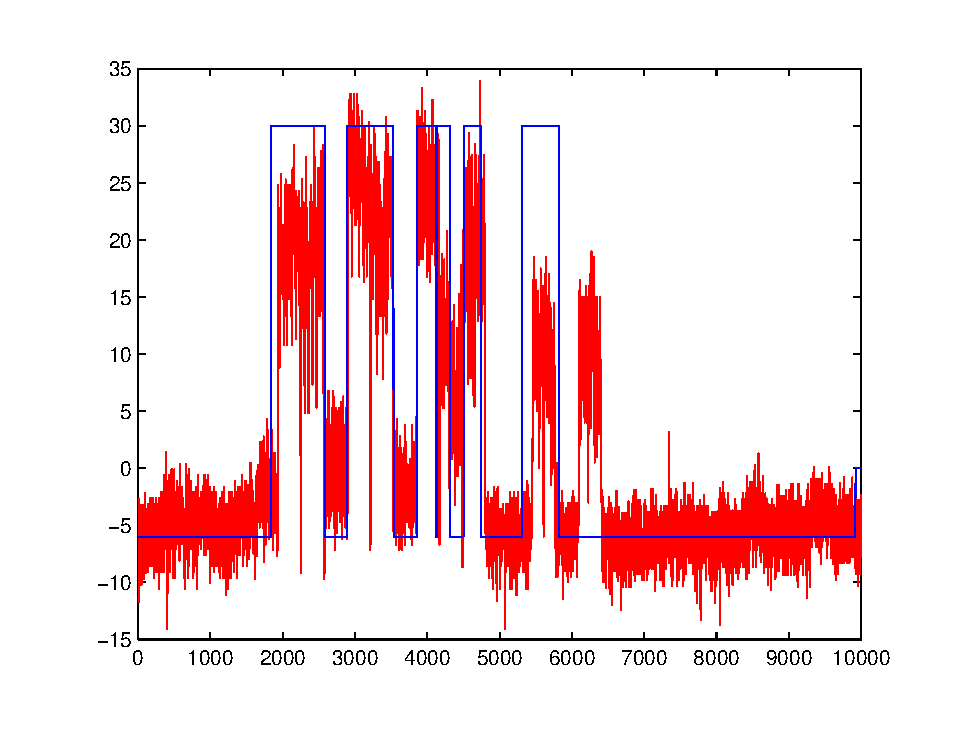
\includegraphics[height = 7.3 cm]{OFCOM6.eps}
\caption{Example of classification with OFCOM data, 55 changepoints}
\label{fig:hvb}
\end{figure}

\begin{figure}[h]
\centering
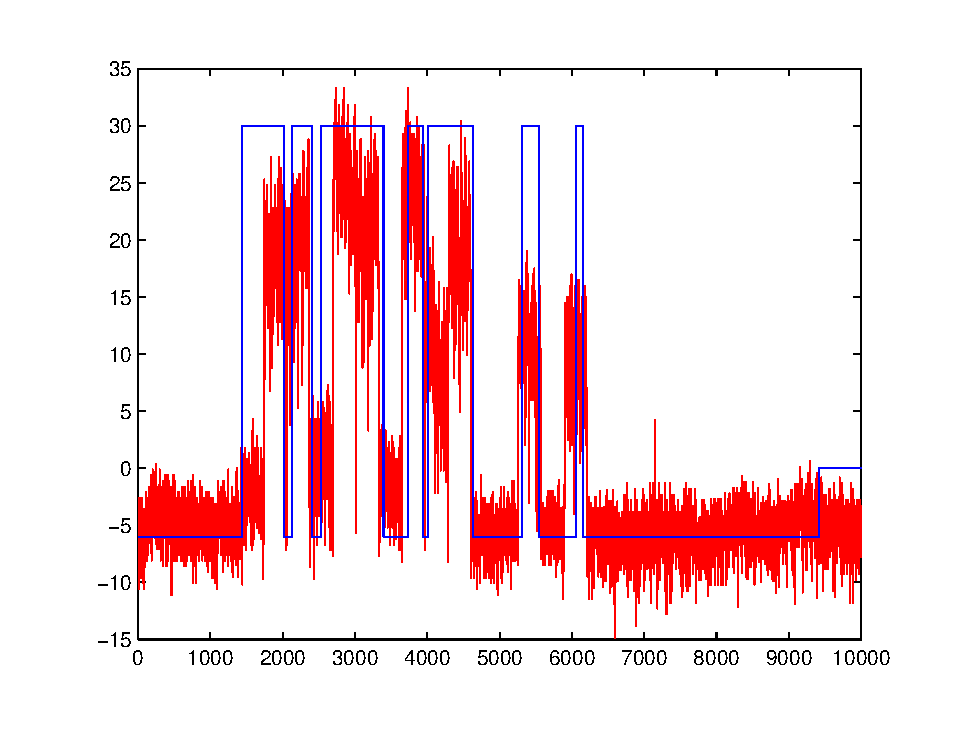
\includegraphics[height = 7.3 cm]{OFCOM7.eps}
\caption{Example of classification with OFCOM data, 35 changepoints}
\label{fig:hvb}
\end{figure}

\begin{figure}[h]
\centering
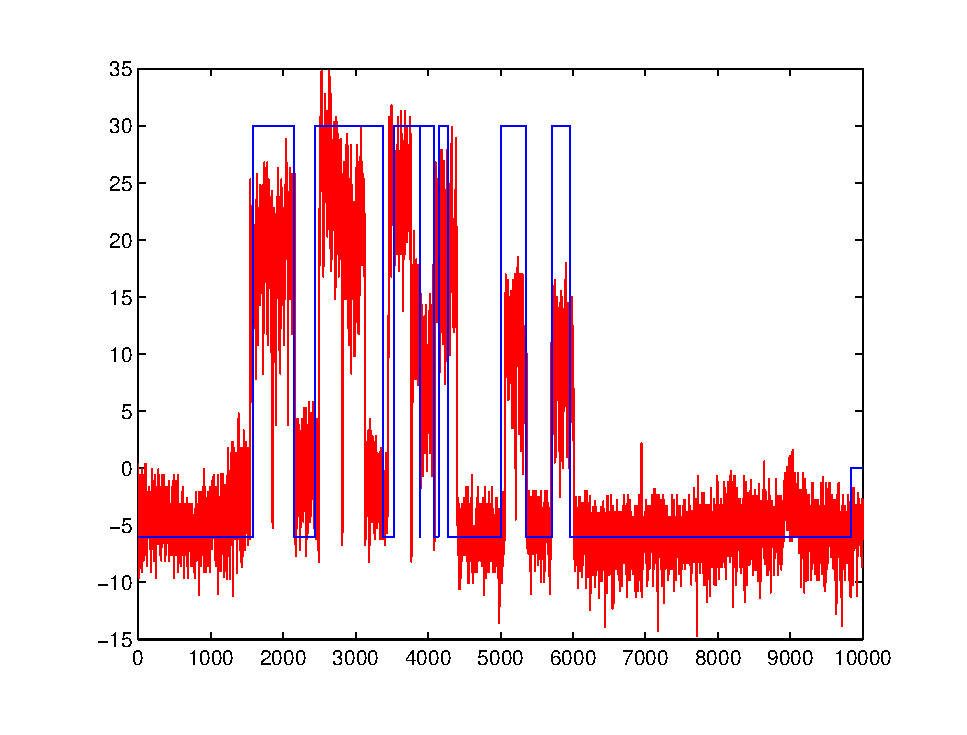
\includegraphics[height = 7.3 cm]{OFCOM8.eps}
\caption{Example of classification with OFCOM data, 55 changepoints}
\label{fig:hvb}
\end{figure}
